\documentclass{beamer}
\usetheme{metropolis}
\usepackage{graphicx}
\usepackage{mathtools}
\usepackage{tcolorbox}
\title{Algebra-Based Physics-2: Electricity, Magnetism, and Modern Physics (PHYS135B-01): Unit 1}
\author{Jordan Hanson}
\institute{Whittier College Department of Physics and Astronomy}

\begin{document}
\maketitle

\section{Summary}

\begin{frame}{Unit 1 Summary}
\textbf{Reading: Chapters 19.4 - 19.7, 20.1 - 20.5, 20.7}
\begin{enumerate}
\item Capacitors and capacitance
\begin{itemize}
\item Equipotential lines
\item Capacitance
\item Capacitors
\end{itemize}
\item Current and DC circuits
\begin{itemize}
\item DC current, resistance, Ohm's law
\item Energy and power in DC current
\item AC current and waveforms
\end{itemize}
\end{enumerate}
\end{frame}

\section{Equipotential Lines and Capacitance}

\begin{frame}{Equipotential Lines}
\small
\textbf{\alert{Equipotential lines}} represent locations of constant potential, and run perpendicular to electric field lines.
\begin{figure}
\centering
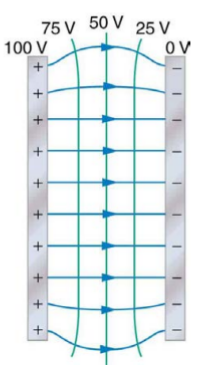
\includegraphics[width=0.2\textwidth]{figures/plates.png}
\caption{\label{fig:plates} Equipotential lines in a parallel plate capacitor.}
\end{figure}
PhET \textit{demonstration}: \\ \url{https://phet.colorado.edu/en/simulations/charges-and-fields}
\end{frame}

\begin{frame}{Capacitance}
What voltage is required to store $Q$? Let $\Delta V$ be the voltage difference, $E$ be the electric field strength, and $\Delta x$ be the capacitor voltage.  We already know that
\begin{equation}
\Delta V = E\Delta x
\end{equation}
We observe that the voltage is linear, so the E-field is constant and proportional to charge per unit area\footnote{Professor: we can prove this if time permits.}
\begin{equation}
E = \frac{\sigma}{\epsilon_0} = \frac{Q}{\epsilon_0 A}
\end{equation}
Substitute $E$ for $Q/(\epsilon_0 A)$, and solve for $Q$:
\begin{equation}
Q = \left( \frac{\epsilon_0 A}{\Delta x} \right) \Delta V
\end{equation}
The term in parentheses is called \textit{the capacitance, C.} \vspace{0.5cm}
\end{frame}

\begin{frame}{Capacitance}
Let the capacitor have an area $A$, and plate separation $d$.  The capacitance is
\begin{align}
C &= \frac{\epsilon_0 A}{d} \\
Q &= C \Delta V
\end{align}
\textit{Capacitance} epresents the ability to store charge.  The unit of capacitance is \textbf{the farad}, after Michael Faraday (encounter mid-semester).  Scaling problems in a moment...
\end{frame}

\section{PhET Activity: Capacitor Basics}

\begin{frame}
\small
Go to the activity: \\ \vspace{0.5cm}
\url{https://phet.colorado.edu/en/simulation/capacitor-lab-basics}
\begin{enumerate}
\item Go to the capacitance tab to find a capacitor and battery.
\item Charge the capacitor under different conditions: $d=10$ mm, $d=2$ mm, $A=100$ mm$^2$, $A=400$ mm$^2$.
\item The \textbf{voltmeter} at right is the yellow and black tool.  It allows the measurement of voltage between two points.  Measure the battery voltage and the capacitor voltage.  Why are they equal?
\item What is the charge stored for $d=2$ mm, and $A=400$ mm$^2$?
\item The light bulb tab in the bottom center contains a circuit that operates a light bulb with the energy stored in the capacitor.  Measure the voltage across the lightbulb as it is powered with the capacitor.  Sketch the voltage as a function of time.
\end{enumerate}
\end{frame}

\begin{frame}{Capacitance}
Two capacitors store the same charge.  One only needs half the voltage, though.  What is true of the capacitor with the lower voltage?
\begin{itemize}
\item A: It has half the capacitance
\item B: It has the same capacitance but more charges
\item C: It has twice the capacitance
\item D: It has half the energy
\end{itemize}
\end{frame}

\begin{frame}{Capacitance}
Two capacitors have the same capacitance.  Capacitor 1 has half the area $A$ as capacitor 2.  Which of the following is true of capacitor 2?
\begin{itemize}
\item A: The plates are half the distance ($\Delta x$) apart
\item B: The plates are twice the distance ($\Delta x$) apart
\item C: The plates have half the voltage
\item D: The plates have twice the voltage
\end{itemize}
\end{frame}

\begin{frame}{Capacitance}
Two identical capacitors power two light bulbs.  Capacitor 1 powers the bulb for 20 seconds, and capacitor 2 powers the bulb for 10 seconds.  Which of the following is true?
\begin{itemize}
\item A: Capacitor 1 was charged at a lower voltage than capacitor 2
\item B: Capacitor 1 was charged at the same voltage as capacitor 2
\item C: Capacitor 1 was charged at a higher voltage than capacitor 2
\item D: Capacitor 2 was not charged
\end{itemize}
\end{frame}

\section{PhET Activity: Capacitor Lab}

\begin{frame}{PhET Activity: Capacitor Lab}
Similar to \textit{Capacitor basics} activity: \\ \vspace{0.5cm}
\url{https://phet.colorado.edu/en/simulations/circuit-construction-kit-ac} \\ \vspace{0.5cm}
\textbf{What is the relationship between total capacitance and individual capacitances?}
\begin{enumerate}
\item How do capacitors add \textit{in series}?
\item How do capacitors add \textit{in parallel}?
\end{enumerate}
\end{frame}

\begin{frame}{PhET Activity: Capacitor Lab}
\small
\textbf{Instructions}:
\begin{enumerate}
\item Click the Lab tab.  Click and drag three capacitors from the white column at left into the main area.
\item Click on each capacitor and minimize the capacitance to 0.05 F.
\item Orient each capacitor \textit{vertically}, and connect the top sides of the capacitors with wires.
\item Connect the bottom sides of the capacitors with wires.
\item Click and drag a battery from the white column at left into the main area, and do the same for a switch.
\item Connect the battery to the first capacitor, and add a switch between the battery and first capacitor.
\item Leave the switch open.
\end{enumerate}
\end{frame}


\begin{frame}{PhET Activity: Capacitor Lab}
\begin{figure}
\centering
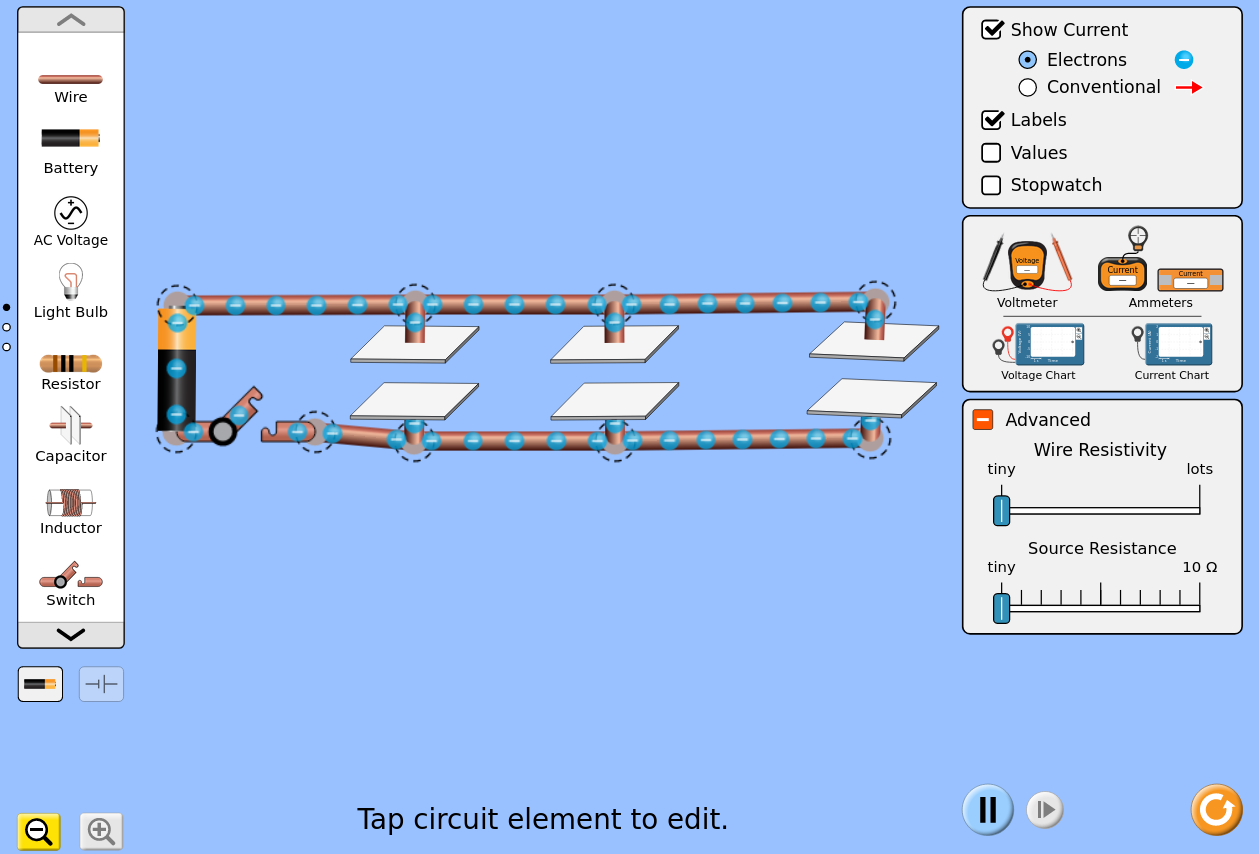
\includegraphics[width=0.8\textwidth]{figures/three_cap.png}
\caption{\label{fig:phet_cap} Three capacitors connected in parallel.}
\end{figure}
\end{frame}

\begin{frame}{PhET Activity: Capacitor Lab}
\small
\textbf{Instructions}:
\begin{enumerate}
\item Click and drag a light bulb from the white column at left, and use wires to connect it to the final capacitor via a switch.
\item Leave both switches open.  If your capacitors are charged, close the light bulb switch until the capacitors are fully discharged.
\item With both switches open, close the battery switch to charge the capacitor.
\item Click and drag the voltage charge tool from the white column at right, and place the red and black probes on either side of the light bulb.
\end{enumerate}
\end{frame}

\begin{frame}{PhET Activity: Capacitor Lab}
\begin{figure}
\centering
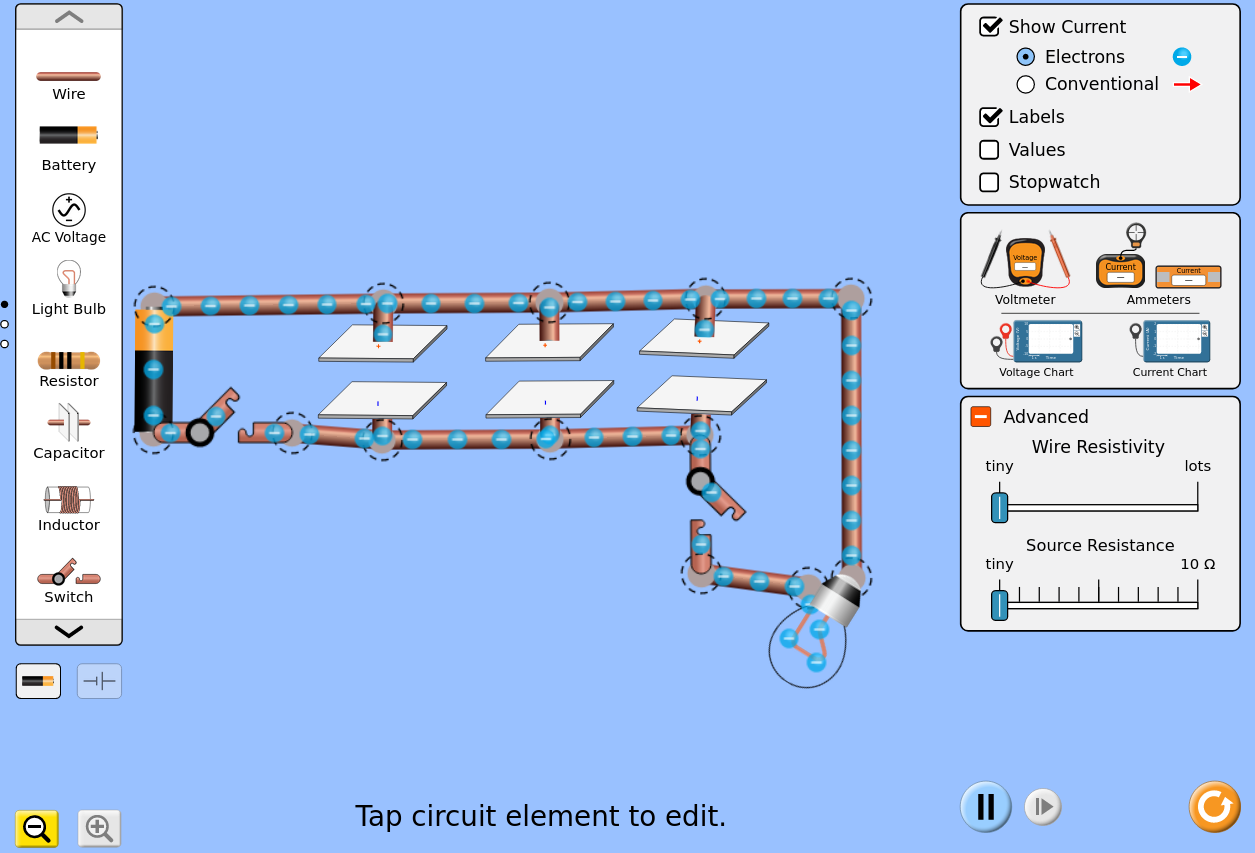
\includegraphics[width=0.8\textwidth]{figures/three_cap_2.png}
\caption{\label{fig:phet_cap2} Three capacitors in parallel, with light and switch.}
\end{figure}
\end{frame}

\begin{frame}{PhET Activity: Capacitor Lab}
\small
\textbf{Instructions}:
\begin{enumerate}
\item Click stopwatch in the white column on the right side.
\item Use the \textbf{\alert{voltage chart}} tool to measure \textit{how long} it takes for the bulb to drain the three capacitors, according to the chart and stopwatch.
\begin{enumerate}
\item Since your capacitors are charged, leave the battery switch open and close the light bulb switch.  Just after closing the switch, click the play button on the stopwatch.
\item Measure the average time required for the bulb voltage to drop to zero by collecting 10 measurements.
\end{enumerate}
\end{enumerate}
\end{frame}

\begin{frame}{PhET Activity: Capacitor Lab}
\small
\textbf{Instructions}:
\begin{enumerate}
\item Now we will repeat the same experiment, but with the capacitors connected \textit{in series.}
\item Rearrange the circuit so that the bottom of the first capacitor connects to the top of the second, and the bottom of the second connects to the top of the third.  Connect the bulb to the bottom capacitor, and add a switch to the other side of the bulb.
\item Connect the top of the top capacitor to the switch, but leave the switch open.
\item Using separate wires, connect the battery to the top and bottom of the circuit, and add a switch to one side of the battery.  Leave both switches open.
\end{enumerate}
\end{frame}

\begin{frame}{PhET Activity: Capacitor Lab}
\begin{figure}
\centering
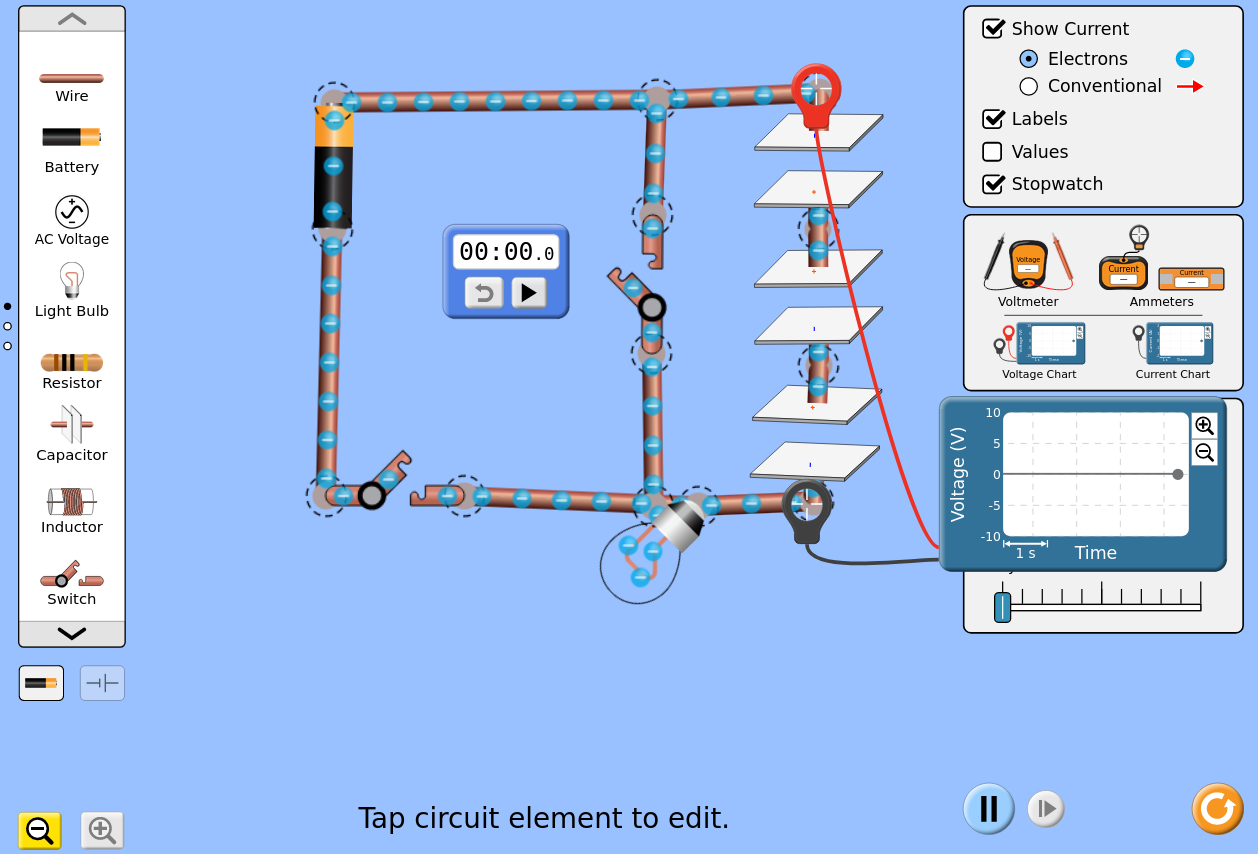
\includegraphics[width=0.8\textwidth]{figures/three_cap_3.png}
\caption{\label{fig:phet_cap3} Three capacitors in series, with light and switch.}
\end{figure}
\end{frame}

\begin{frame}{PhET Activity: Capacitor Lab}
\begin{enumerate}
\item Use the \textbf{\alert{voltage chart}} tool to measure \textit{how long} it takes for the bulb to drain the three capacitors, according to the chart and stopwatch.
\begin{enumerate}
\item Charge the capacitors by closing the battery switch, and then leave it open.
\item Close the light bulb switch.  Measure the average time required for the bulb voltage to drop to zero by collecting 10 measurements.
\end{enumerate}
\item Which capacitor arrangement takes longer to drain?
\item Given that we used the same voltage for both arrangements, which arrangement (parallel or series) stores more charge?
\end{enumerate}
\end{frame}

\section{Energy in Capacitors}

\begin{frame}{Energy in Capacitors}
Energy stored in a \textit{an electric field}, E:
\begin{equation}
\mathcal{E} = \frac{1}{2} \epsilon_0 E^2 \label{eq:energy}
\end{equation}
The proof of Eq. \ref{eq:energy} will come later in the course.  We also know that the E-field is constant because the voltage is linear.  In a parallel-plate capacitor, $E=\sigma/\epsilon_0 = Q/(\epsilon_0 A)$. Use $Q = C V$ and Eq. \ref{eq:energy} to show that the total energy in a capacitor with capacitance $C$ is 
\begin{align}
U_C &= \frac{1}{2} \frac{Q^2}{C} \\
U_C &= \frac{1}{2} CV^2
\end{align}
\textbf{Observe proof on board.} The variable $\sigma$ is known as the \textit{surface charge density.}
\end{frame}

\begin{frame}{Energy in Capacitors}
Suppose we have a 10 nF capacitor at 5V.  How many Joules are stored in it?
\begin{itemize}
\item A: 100 nJ
\item B: 100 pJ
\item C: 125 nJ
\item D: 125 pJ
\end{itemize}
\end{frame}

\section{Capacitors, Series and Parallel}

\begin{frame}{Capacitors, Series and Parallel}
\begin{figure}
\centering
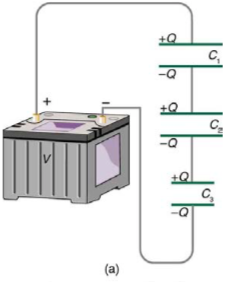
\includegraphics[width=0.3\textwidth]{figures/cap1.png} \hspace{0.2cm}
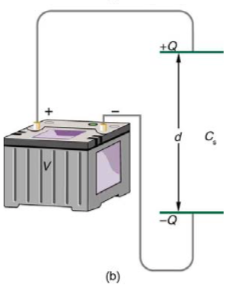
\includegraphics[width=0.3\textwidth]{figures/cap2.png}
\caption{\label{fig:cap} How do we compute the total capacitance of (a) such that we know the charge stored for a given voltage in (b)?}
\end{figure}
\end{frame}

\begin{frame}{Capacitors, Series and Parallel}
\small
Notice that \textit{charge is conserved}, so $Q$ has to be the same on all capacitors
But that means the \textit{voltage} on the different capacitors has to obey
\begin{align}
Q &= Q_1 = Q_2 = Q_3 \\
C_{\rm tot} V_{\rm tot} &= C_1 V_1 = C_2 V_2 = C_3 V_3
\end{align}
To conserve energy, we know that
\begin{align}
V_{\rm tot} &= V_1 + V_2 + V_3 \\
\frac{Q}{C_{\rm tot}} &= \frac{Q}{C_1} + \frac{Q}{C_2} + \frac{Q}{C_3} \\
\Aboxed{\frac{1}{C_{\rm tot}} &= \frac{1}{C_1} + \frac{1}{C_2} + \frac{1}{C_3}}
\end{align}
This is the how that capacitance adds for capacitors \textbf{in series}.
\end{frame}

\begin{frame}{Capacitors, Series and Parallel}
\begin{figure}
\centering
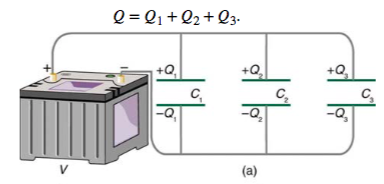
\includegraphics[width=0.4\textwidth]{figures/cap3.png} \hspace{0.2cm}
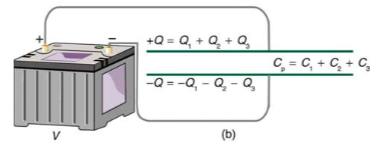
\includegraphics[width=0.4\textwidth]{figures/cap4.png}
\caption{\label{fig:cap2} How do we compute the total capacitance of (a) such that we know the charge stored for a given voltage in (b)?}
\end{figure}
\end{frame}

\begin{frame}{Capacitors, Series and Parallel}
Note that all the capacitors are at the same voltage, because wires are equipotentials.  Thus,
\begin{equation}
V_{\rm tot} = V_1 = V_2 = V_3 = V
\end{equation}
The total charge stored is
\begin{align}
Q_{\rm tot} &= Q_1 + Q_2 + Q_3 \\
C_{\rm tot} V &= C_1 V + C_1 V + C_2 V \\
\Aboxed{C_{\rm total} &= C_1+C_2+C_3}
\end{align}
This is the how that capacitance adds for capacitors \textbf{in parallel}.
\end{frame}

\section{Current}

\begin{frame}{Current}
\underline{Notions of current:}
\begin{itemize}
	\item $I = \frac{\Delta Q}{\Delta t}$ - The derivative of charge
	\item The \textit{movement} of electrons
	\item The \textit{flow} of charge
	\item Number of Coulombs per second (1 Amp = C/s)
\end{itemize}
\begin{columns}[T]
\begin{column}{0.5\textwidth}
Speed of typical electronic signals: $\approx 10^{8}$ m/s
\end{column}
\begin{column}{0.5\textwidth}
Typical speed of actual charges passing through a conductor under voltage: $\approx 10^{-4}$ m/s
\end{column}
\end{columns} \vspace{0.25cm}
\textbf{Since there is a 12 order of magnitude range, it's probably a good idea to ponder...\textbf{Observe proof on board.}}
\end{frame}

\section{Ohm's Law}

\begin{frame}{Ohm's Law}
\small
Energy is transferred to objects that are not perfect conductors in a simple circuit.
\begin{figure}
\centering
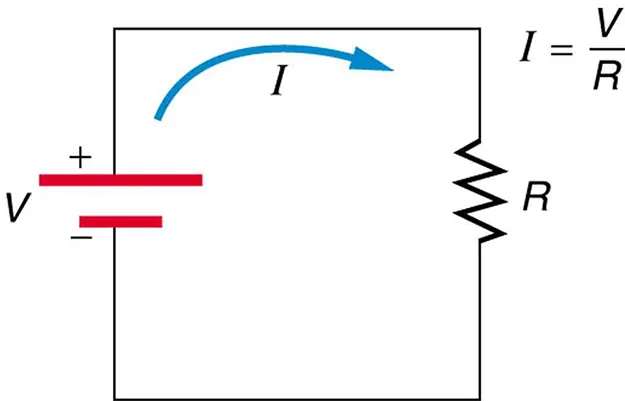
\includegraphics[width=0.4\textwidth]{figures/simple.png}
\caption{\label{fig:simple} Current transfers energy to \textit{resistors}.}
\end{figure}
Ohm's law: for a \textit{resistance} R, the voltage $V$ and the current $i$ are related by:
\begin{equation}
V = i R
\end{equation}
\textbf{Instructor:} Perform a few examples.
\end{frame}

%\section{PhET: DC Circuits and Ohm's Law}
%
%\begin{frame}{Ohm's Law}
%Go to the activity: \url{https://phet.colorado.edu/en/simulation/circuit-construction-kit-dc}
%\end{frame}
%
%\begin{frame}{Current}
%\textbf{\alert{PhET}}: Create a DC circuit involving a battery, resistor (the brown striped object), a light bulb, and a switch.
%\begin{enumerate}
%\item Place the battery and connect to it a wire, and attach a resistor to that wire.
%\item To the other end of the resistor, connect a switch and leave it open.
%\item Connect a light bulb to the other end of the switch, and connect a wire from the light bulb to the battery.
%\item The properties of each circuit element can be edited by clicking on the element.
%\end{enumerate}
%\end{frame}
%
%\begin{frame}{Current}
%\begin{figure}
%\centering
%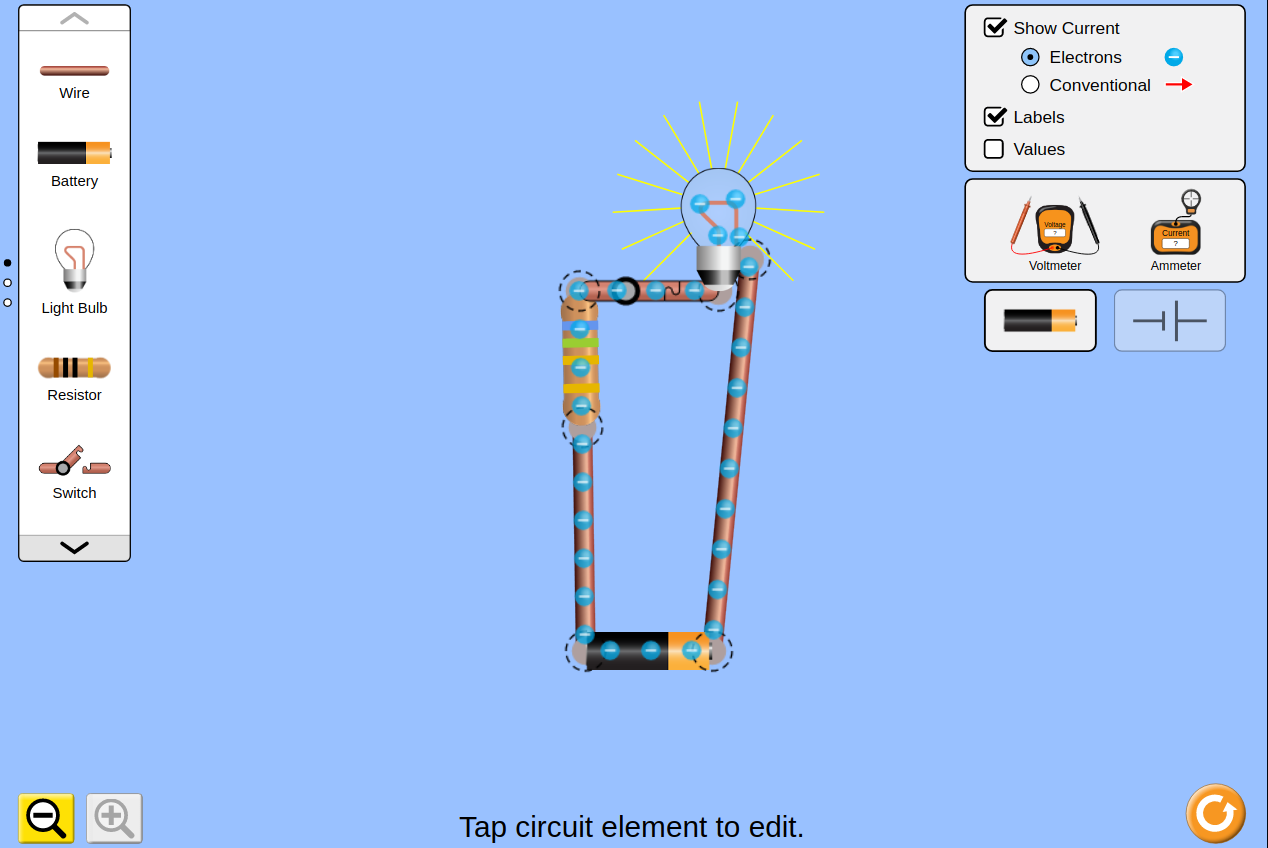
\includegraphics[width=0.75\textwidth]{figures/PhETBulb.png}
%\caption{\label{fig:phetb} Your circuit should resemble this.}
%\end{figure}
%\end{frame}
%
%\begin{frame}{Current}
%\textbf{\alert{PhET}}: Make observations.
%\begin{enumerate}
%\item What happens to the drift velocity of the electrons as you raise and lower the resistance?  Why do we call light bulbs and the brown striped objects ``resistors?''  Make a sketch of what you think the speed vs. resistance is.
%\item How does the current change if you increase the voltage? Make a sketch of what you think the speed vs. voltage is.
%\end{enumerate}
%\end{frame}
%
%\begin{frame}{Current}
%\textbf{\alert{PhET}}: \textbf{The unit of resistance is the Ohm.  We use the symbol $\Omega$ for Ohms, and $1\Omega = 1$V/A.}
%\begin{enumerate}
%\item There are two devices available in the white toolbox on the right-hand side: the \textit{voltmeter}, and the \textit{ammeter}.  Using these devices, measure the voltage drop across the resistor and the light bulb, and the current flowing through the circuit.
%\item For fixed resistance, take 15 measurements of current as you vary the voltage.  Plot voltage vs. current in Excel, and calculate the slope.
%\item What is the number for the slope?  How does it compare to the resistor value?
%\end{enumerate}
%\end{frame}
%
%\begin{frame}{Current}
%\textbf{Ohm's Law}: Let $V$ be the voltage change across a resistor with resistance $R$, and let $i$ be the current flowing through the resistor.  Ohm's law states that
%\begin{equation}
%\boxed{
%V = iR}
%\end{equation}
%for materials that fall into the category of \textit{Ohmic}.
%\end{frame}
%
%\begin{frame}{Current}
%\small
%\textbf{\alert{PhET}}: \textbf{How do we deal with more complex circuits?} There must be a way to ``add'' resistors.
%\begin{enumerate}
%\item Create a circuit that involves two resistors \textit{in series}.
%\item Calculate the \textit{effective total resistance} by plotting an $i-V$ curve of the system.  Measure $i$ and $V$ by changing the voltage and using the voltmeter and ammeter.  What is a rule for obtaining the total resistance for a group of resistors in series?
%\item Create a circuit that involves two resistors \textit{in parallel}.
%\item Calculate the \textit{effective total resistance} by plotting an $i-V$ curve of the system.  Measure $i$ and $V$ by changing the voltage and using the voltmeter and ammeter.   What is a rule for obtaining the total resistance for a group of resistors in parallel?
%\item \textbf{For these exercises, it's helpful to use resistors of the same value.}
%\end{enumerate}
%\end{frame}
%
%\begin{frame}{Current}
%As you may have discovered, \textit{resistors in series} \textbf{add}:
%\begin{equation}
%R_{\rm tot} = R_1 + R_2 + ...
%\end{equation}
%\textit{Resistors in parallel} \textbf{add their reciprocals}:
%\begin{equation}
%\frac{1}{R_{\rm tot}} = \frac{1}{R_1}+\frac{1}{R_2}+...
%\end{equation}
%\end{frame}
%
%\begin{frame}{Current}
%Resitance is not an \textit{intrinsic property} of materials.  Imagine a 0.1 m-long wire (which is a conductor) actually having a small resistance.  What about that same wire, but 1 kilometer long?
%\begin{itemize}
%\item Electrons lose some fixed energy per unit length in a given material (\textit{Joule heating})
%\item Electrons lose more energy if the wire is thinner (\textit{Joule heating})
%\end{itemize}
%\textbf{Resistivity} $\rho$ is defined in terms of resistance $R$, length $L$ and cross-sectional area $A$ as
%\begin{equation}
%R = \rho \left( \frac{L}{A} \right)
%\end{equation}
%\end{frame}
%
%\begin{frame}{Current}
%\begin{columns}[T]
%\begin{column}{0.5\textwidth}
%\begin{figure}
%\centering
%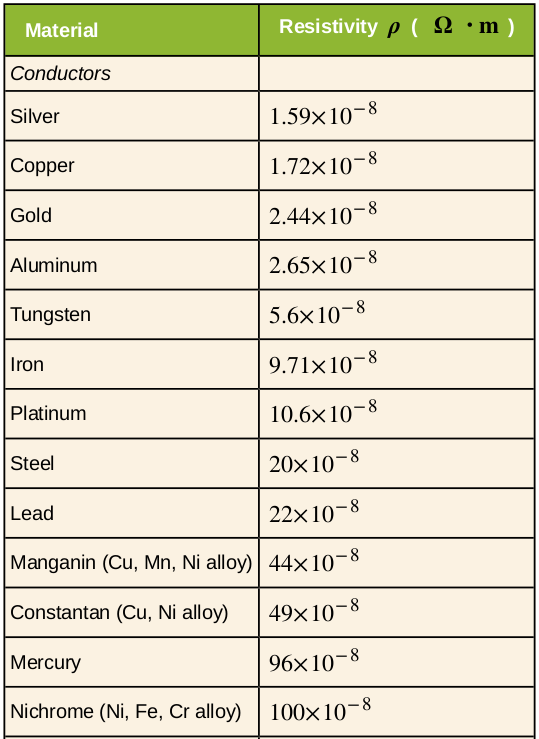
\includegraphics[width=0.7\textwidth]{figures/rho1.png}
%\caption{\label{fig:rho1} Conductor resistivities are in units of $\Omega$ m, and are small but non-zero.}
%\end{figure}
%\end{column}
%\begin{column}{0.5\textwidth}
%\begin{figure}
%\centering
%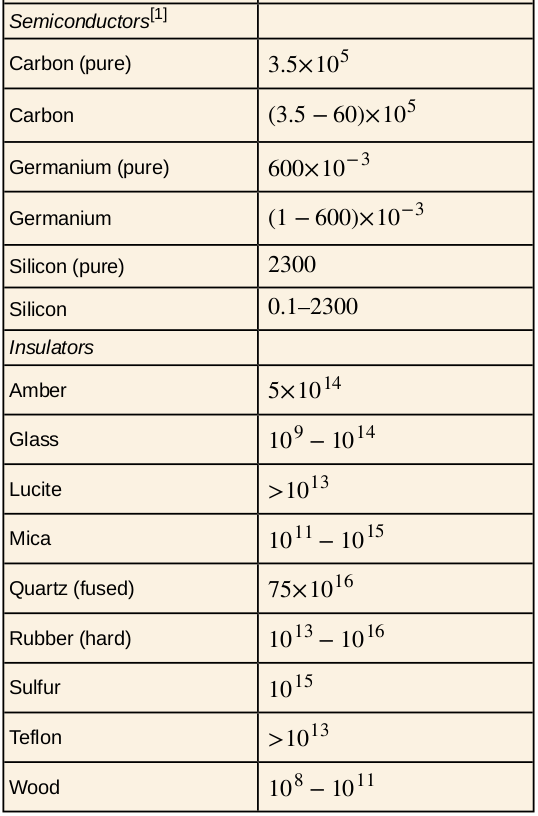
\includegraphics[width=0.7\textwidth]{figures/rho2.png}
%\caption{\label{fig:rho2} Semiconductor resistivities are in units of $\Omega$ m, and are larger.}
%\end{figure}
%\end{column}
%\end{columns}
%\end{frame}
%
%\begin{frame}{Current}
%A copper wire carrying current to the top floor of a building, that has a cross-sectional area of 12 mm$^2$ and is 10 meters long.  The resistivity of copper is $1.7 \times 10^{-8}$ $\Omega$ m.  What is the resistance of the wire?
%\begin{itemize}
%\item A: about 1 m$\Omega$
%\item B: about 10 m$\Omega$
%\item C: about 100 m$\Omega$
%\item D: about 1 $\Omega$
%\end{itemize}
%\end{frame}
%
%\begin{frame}{Current}
%Consider the same system.  If we attach a battery and use the wire to feed voltage to some circuit drawing 3.0 A of current, what is the voltage drop due to just the wire?
%\begin{itemize}
%\item A: about 30 mV
%\item B: about 300 mV
%\item C: about 3 V
%\item D: Current will not flow at all
%\end{itemize}
%\end{frame}
%
%\begin{frame}{Current}
%What would the resistance be if the wire system was 10 times as long?
%\begin{itemize}
%\item A: about 30 mV
%\item B: about 300 mV
%\item C: about 3 V
%\item D: Current will not flow at all
%\end{itemize}
%\textit{So you can start to see that resistance matters even for conductors, if the current is traveling for long distances.  Often manufacturers quote the Ohms per foot in wire data sheets.}
%\end{frame}
%
%\begin{frame}{Current}
%Resistivity depends on temperature in the following way:
%\begin{equation}
%\rho = \rho_{\rm 0} \left(1 + \alpha \Delta T\right)
%\end{equation}
%For most conductors, $\alpha$ is small, on the order of $10^{-3}$ $^\circ$C$^{-1}$.
%\end{frame}
%
%\begin{frame}{Current}
%\begin{figure}
%\centering
%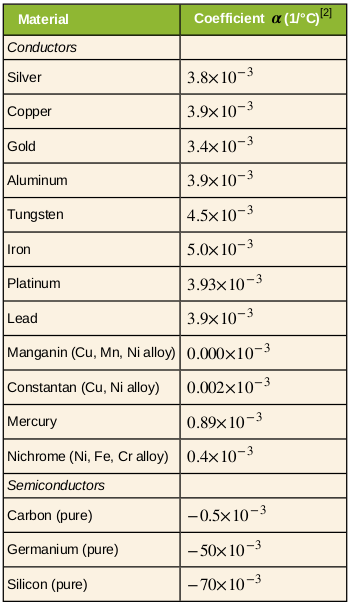
\includegraphics[width=0.35\textwidth]{figures/rho3.png}
%\caption{\label{fig:rho3} Conductor resistivities depend on temperature.}
%\end{figure}
%\end{frame}
%
%\begin{frame}{Current}
%Continuing with the same example of the long copper wire with $R = 10$ m$\Omega$, if the temperature increases by 50.0 deg C, what is the new resistance? ($\alpha = 3.9 \times 10^{-3}$ $^{\circ}$C$^{-1}$).
%\begin{itemize}
%\item A: 8 m$\Omega$
%\item B: 12 m$\Omega$
%\item C: 18 m$\Omega$
%\item D: 22 m$\Omega$
%\end{itemize}
%\end{frame}
%
%\section{Graphical Analysis of Simple Circuits}
%
%\begin{frame}{Graphical Analysis of Simple Circuits}
%\begin{columns}[T]
%\begin{column}{0.5\textwidth}
%\begin{figure}
%\centering
%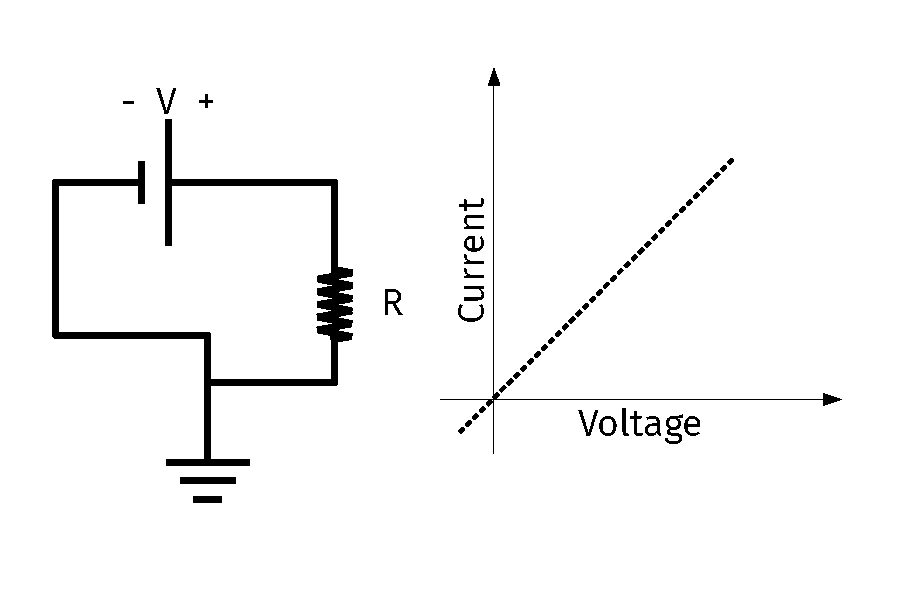
\includegraphics[width=\textwidth,trim=0.5cm 0cm 1cm 0cm,clip=true]{figures/iVCurve.pdf}
%\caption{\label{fig:iVCurve1} Circuits components are represented graphically by iV curves.}
%\end{figure}
%\end{column}
%\begin{column}{0.5\textwidth}
%\small
%If the resistance $R$ is increased, what will happen?
%\begin{itemize}
%\item A: The slope on the graph will increase
%\item B: The slope on the graph will decrease
%\item C: The slope will stay the same
%\item D: Cannot determine what will happen
%\end{itemize}
%\end{column}
%\end{columns}
%\end{frame}
%
%\begin{frame}{Graphical Analysis of Simple Circuits}
%\begin{columns}[T]
%\begin{column}{0.5\textwidth}
%\begin{figure}
%\centering
%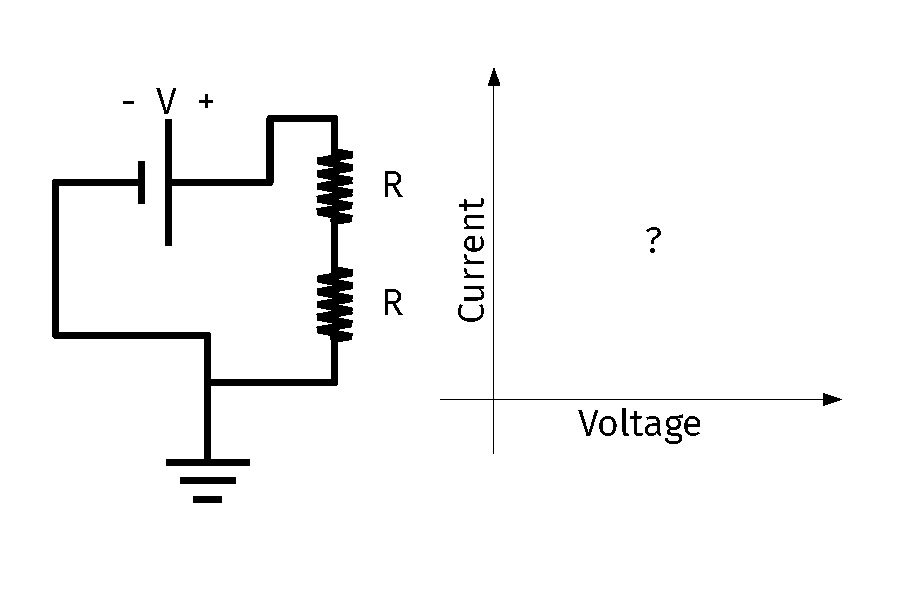
\includegraphics[width=\textwidth,trim=0.5cm 0cm 1cm 0cm,clip=true]{figures/iVCurve2.pdf}
%\caption{\label{fig:iVCurve2} Circuits components are represented graphically by iV curves.}
%\end{figure}
%\end{column}
%\begin{column}{0.5\textwidth}
%\small
%Should the slope now be greater than, less than, or equal to the that of Fig. \ref{fig:iVCurve1}?
%\begin{itemize}
%\item A: Greater than Fig. \ref{fig:iVCurve1}
%\item B: Less than Fig. \ref{fig:iVCurve1}
%\item C: Equal to Fig. \ref{fig:iVCurve1}
%\item D: Cannot determine.
%\end{itemize}
%\end{column}
%\end{columns}
%\end{frame}
%
%\begin{frame}{Graphical Analysis of Simple Circuits}
%\begin{columns}[T]
%\begin{column}{0.5\textwidth}
%\begin{figure}
%\centering
%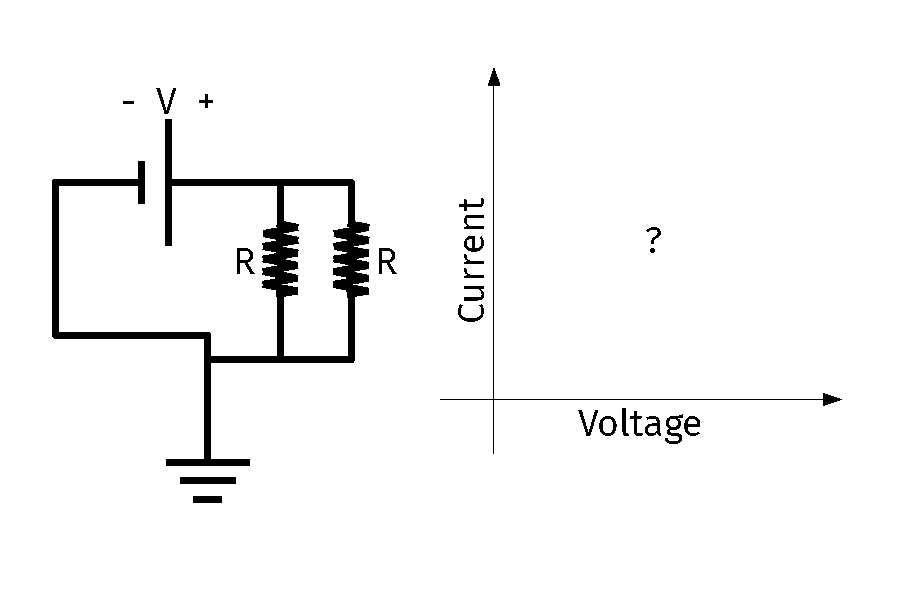
\includegraphics[width=\textwidth,trim=0.5cm 0cm 1cm 0cm,clip=true]{figures/iVCurve3.pdf}
%\caption{\label{fig:iVCurve3} Circuits components are represented graphically by iV curves.}
%\end{figure}
%\end{column}
%\begin{column}{0.5\textwidth}
%\small
%Should the slope now be greater than, less than, or equal to the that of Fig. \ref{fig:iVCurve1}?
%\begin{itemize}
%\item A: Greater than Fig. \ref{fig:iVCurve1}
%\item B: Less than Fig. \ref{fig:iVCurve1}
%\item C: Equal to Fig. \ref{fig:iVCurve1}
%\item D: Cannot determine.
%\end{itemize}
%\end{column}
%\end{columns}
%\end{frame}
%
%\begin{frame}{Graphical Analysis of Simple Circuits}
%\begin{columns}[T]
%\begin{column}{0.5\textwidth}
%\begin{figure}
%\centering
%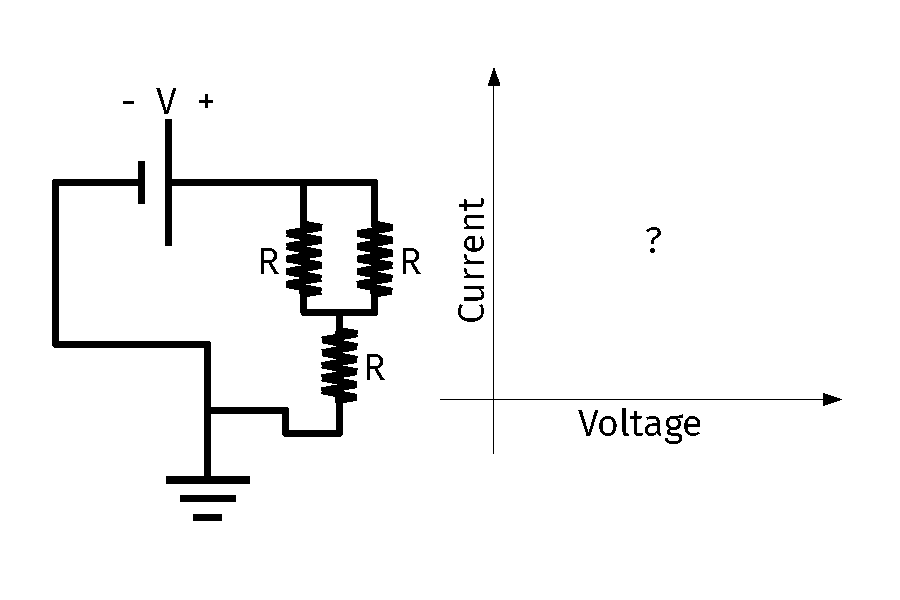
\includegraphics[width=\textwidth,trim=0.5cm 0cm 1cm 0cm,clip=true]{figures/iVCurve4.pdf}
%\caption{\label{fig:iVCurve4} Circuits components are represented graphically by iV curves.}
%\end{figure}
%\end{column}
%\begin{column}{0.5\textwidth}
%\small
%Should the slope now be greater than, less than, or equal to the that of Fig. \ref{fig:iVCurve1}?
%\begin{itemize}
%\item A: Greater than Fig. \ref{fig:iVCurve1}
%\item B: Less than Fig. \ref{fig:iVCurve1}
%\item C: Equal to Fig. \ref{fig:iVCurve1}
%\item D: Cannot determine.
%\end{itemize}
%\end{column}
%\end{columns}
%\end{frame}
%
%\section{Power}
%
%\begin{frame}{Current}
%Recall that \textbf{power} is consumed in resistors, since charges are losing energy and new charges are showing up at a certain rate.  Consider the PE converted to work in a resistor:
%\begin{align}
%\Delta PE =& \Delta q\Delta V \\
%\Delta W =& \Delta q i R \\
%\frac{\Delta W}{\Delta t} =& \frac{\Delta q}{\Delta t} i R = i^2 R \\
%\frac{\Delta W}{\Delta t} =& i V \\
%P =& iV
%\end{align}
%The formula $P = iV$ shows that the wattage required by some device in a circuit will pull current according to the voltage of the battery.
%\end{frame}
%
%\begin{frame}{Current}
%How much current is required by a 50 W light bulb if the voltage supplying it is 120 V?
%\begin{itemize}
%\item A: 420 mA
%\item B: 120 mA
%\item C: 50 mA
%\item D: 50 V
%\end{itemize}
%\end{frame}
%
%\begin{frame}{Graphical Analysis of Simple Circuits}
%A \textit{fuse} is a device that disconnects a circuit if the current rises above a pre-defined value.  Some fuses have a wire that is rated to melt at a given current such that the circuit is no longer closed.  Suppose a deviced rated to consume 50 W is connected to a 12 V battery, in series with a fuse that is rated to blow at 1 A.  Does it blow?
%\begin{itemize}
%\item A: Yes
%\item B: No
%\item C: WAT
%\end{itemize}
%\end{frame}
%
%\begin{frame}{Current}
%Suppose a deviced rated to consume 50 W is connected to a 12 V battery, and a second identical device is connected in parallel to it.  In series with these devices and the battery is a fuse that is rated to blow at 5 A.  Does it blow?
%\begin{itemize}
%\item A: Yes
%\item B: No
%\item C: WAT
%\end{itemize}
%\end{frame}
%
%\begin{frame}{Current}
%\begin{columns}[T]
%\begin{column}{0.5\textwidth}
%\begin{figure}
%\centering
%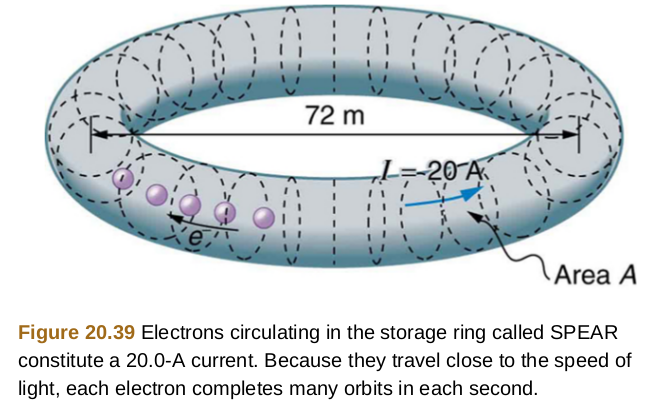
\includegraphics[width=\textwidth]{figures/SPEAR.png}
%\caption{\label{fig:SLAC} A component of the Stanford Linear Accelerator (SLAC) stores high-energy electrons.}
%\end{figure}
%\end{column}
%\begin{column}{0.5\textwidth}
%\small
%SPEAR, a storage ring about 72.0 m in diameter at the Stanford Linear Accelerator (closed in 2009), has a 200.0-A circulating beam of electrons that are moving at nearly the speed of light. (See Figure 20.39.) How many electrons are in the beam?
%\begin{itemize}
%\item A: $10^{11}$
%\item B: $10^{12}$
%\item C: $10^{13}$
%\item D: $10^{14}$
%\end{itemize}
%\end{column}
%\end{columns}
%\end{frame}
%
%\begin{frame}{Current}
%\begin{columns}[T]
%\begin{column}{0.5\textwidth}
%\begin{figure}
%\centering
%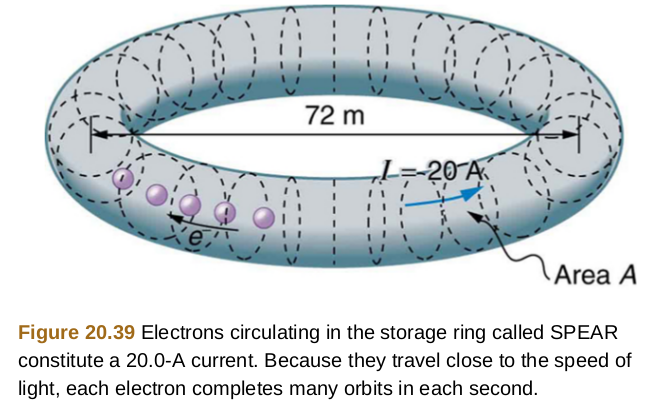
\includegraphics[width=\textwidth]{figures/SPEAR.png}
%\caption{\label{fig:SLAC2} A component of the Stanford Linear Accelerator (SLAC) stores high-energy electrons.}
%\end{figure}
%\end{column}
%\begin{column}{0.5\textwidth}
%\small
%Suppose each electron was dropped through a potential of 1 kV as it enters the ring.  What is the energy of each electron?
%\begin{itemize}
%\item A: 100 eV
%\item B: 1 keV
%\item C: 1 MeV
%\item D: 1 Joule
%\end{itemize}
%\end{column}
%\end{columns}
%\end{frame}
%
%\begin{frame}{Current}
%\begin{columns}[T]
%\begin{column}{0.5\textwidth}
%\begin{figure}
%\centering
%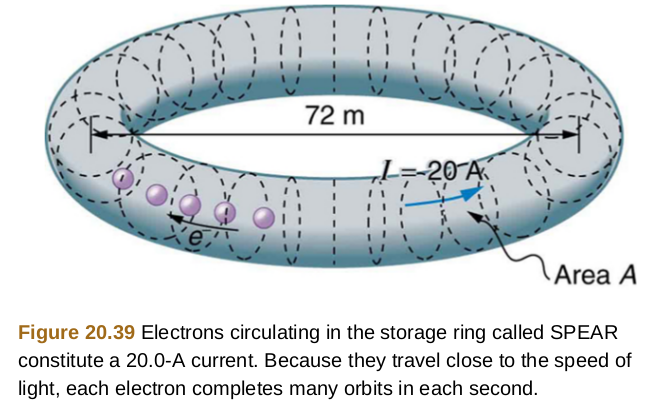
\includegraphics[width=\textwidth]{figures/SPEAR.png}
%\caption{\label{fig:SLAC3} A component of the Stanford Linear Accelerator (SLAC) stores high-energy electrons.}
%\end{figure}
%\end{column}
%\begin{column}{0.5\textwidth}
%\small
%What's the total energy of all the electrons?  (Multiply the previous two answers).
%\begin{itemize}
%\item A: $10^{16}$ eV
%\item B: $10^{17}$ eV
%\item C: $10^{18}$ eV
%\item D: $10^{19}$ eV
%\end{itemize}
%\end{column}
%\end{columns}
%\end{frame}
%
%\begin{frame}{Current}
%\begin{columns}[T]
%\begin{column}{0.5\textwidth}
%\begin{figure}
%\centering
%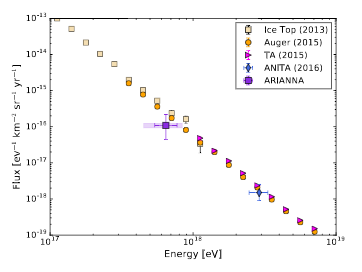
\includegraphics[width=0.9\textwidth]{figures/ARIANNA1.png}
%\caption{\label{fig:ARIANNA1} Cosmic ray protons' flux observed recently by the ARIANNA experiment.}
%\end{figure}
%\end{column}
%\begin{column}{0.5\textwidth}
%\small
%How much energy is $10^{17}$ eV?  Recently, the ARIANNA experiment observed protons with so much energy (about $5-9 \times 10^{17}$ eV) the ensuing shock in the atmosphere created a radio pulse observed over a several kilometer range.
%\end{column}
%\end{columns}
%\end{frame}
%
%\begin{frame}{Current}
%\begin{columns}[T]
%\begin{column}{0.5\textwidth}
%\begin{figure}
%\centering
%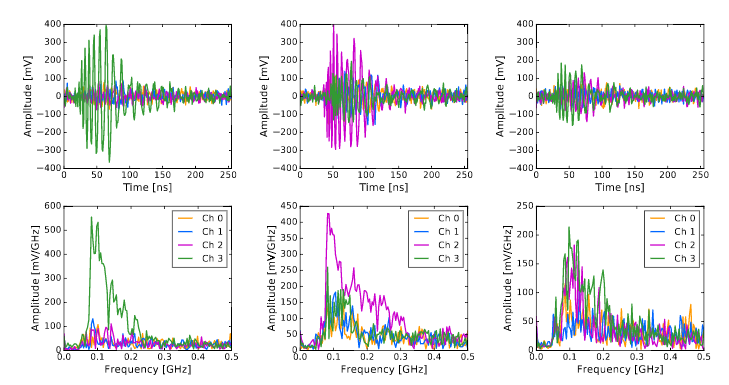
\includegraphics[width=0.95\textwidth]{figures/ARIANNA2.png}
%\caption{\label{fig:ARIANNA2} Cosmic ray protons' flux observed recently by the ARIANNA experiment.}
%\end{figure}
%\end{column}
%\begin{column}{0.5\textwidth}
%\small
%How much energy is $10^{17}$ eV?  Recently, the ARIANNA experiment observed protons with so much energy (about $5-9 \times 10^{17}$ eV) the ensuing shock in the atmosphere created a radio pulse observed over a several kilometer range.
%\end{column}
%\end{columns}
%\end{frame}
%
%\begin{frame}{Current}
%\begin{columns}[T]
%\begin{column}{0.5\textwidth}
%\begin{figure}
%\centering
%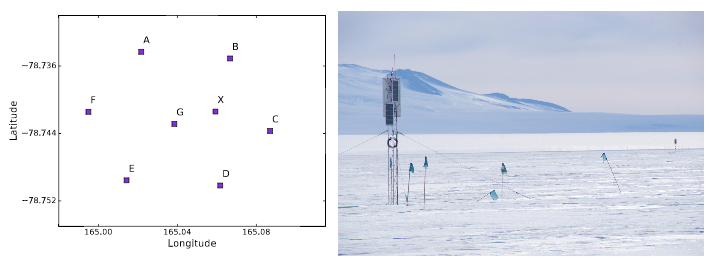
\includegraphics[width=0.9\textwidth]{figures/ARIANNA3.png}
%\caption{\label{fig:ARIANNA3} Cosmic ray protons' flux observed recently by the ARIANNA experiment.}
%\end{figure}
%\end{column}
%\begin{column}{0.5\textwidth}
%\small
%How much energy is $10^{17}$ eV?  Recently, the ARIANNA experiment observed protons with so much energy (about $5-9 \times 10^{17}$ eV) the ensuing shock in the atmosphere created a radio pulse observed over a several kilometer range.
%\end{column}
%\end{columns}
%\textbf{Good paper topic:} What is the purpose of the ARIANNA and ARA experiments in the Antarctic?  What are they trying to measure? \\
%\textbf{Stay tuned for CON2 course in the Fall:} The History and Current Status of Science in Antarctica
%\end{frame}

\section{Conclusion}

\begin{frame}{Unit 1 Summary}
\textbf{Reading: Chapters 19.4 - 19.7, 20.1 - 20.5, 20.7}
\begin{enumerate}
\item Capacitors and capacitance
\begin{itemize}
\item Equipotential lines
\item Capacitance
\item Capacitors
\end{itemize}
\item Current and DC circuits
\begin{itemize}
\item DC current, resistance, Ohm's law
\item Energy and power in DC current
\item AC current and waveforms
\end{itemize}
\end{enumerate}
\end{frame}

\end{document}
